\section{Design Options}
\label{sec:options}

The nose is defined by three choices: the \textbf{profile family}, the \textbf{fineness}
$L/D$ (curved length over base diameter) and the \textbf{tip bluntness} $r_n/R$. Seven
profiles are compared (Figure~\ref{fig:profiles}). With $\xi = x/L$ and $\eta = y/R$:

\begin{table}[H]
\centering
\caption{Candidate profiles. $x_{cp}$: Barrowman nose centre of pressure; $\theta_{\rm sh}$: angle
to the body at the shoulder (0 = tangent).}
\label{tab:profiles}
\small
\begin{adjustbox}{max width=\textwidth}
\begin{tabular}{@{}lllcc@{}}
\toprule
Profile & $\eta(\xi)$ & ERT heritage & $x_{cp}/L$ & $\theta_{\rm sh}$ at $L/D=4$ \\
\midrule
Conical & $\xi$ & -- & 0.667 & $7.1^\circ$ \\
Tangent ogive & $\sqrt{\rho^2-(L-x)^2}+R-\rho$, $\rho=\frac{R^2+L^2}{2R}$ & Bella Lui II, Nordend & 0.464 & $0^\circ$ \\
Parabolic ($K'=1$) & $2\xi-\xi^2$ & -- & 0.467 & $0^\circ$ \\
Power series $n=\tfrac12$ & $\xi^{1/2}$ & Wildhorn, Firehorn & 0.500 & $3.6^\circ$ \\
Power series $n=\tfrac34$ & $\xi^{3/4}$ & -- & 0.600 & $5.4^\circ$ \\
LV-Haack ($C=\tfrac13$) & $\pi^{-1/2}\sqrt{\theta-\tfrac12\sin2\theta+C\sin^3\theta}$, $\theta=\arccos(1-2\xi)$ & -- & 0.438 & $0^\circ$ \\
Von K\'arm\'an ($C=0$) & as LV-Haack with $C=0$ & -- & 0.500 & $0^\circ$ \\
\bottomrule
\end{tabular}
\end{adjustbox}
\end{table}

\begin{figure}[H]
\centering
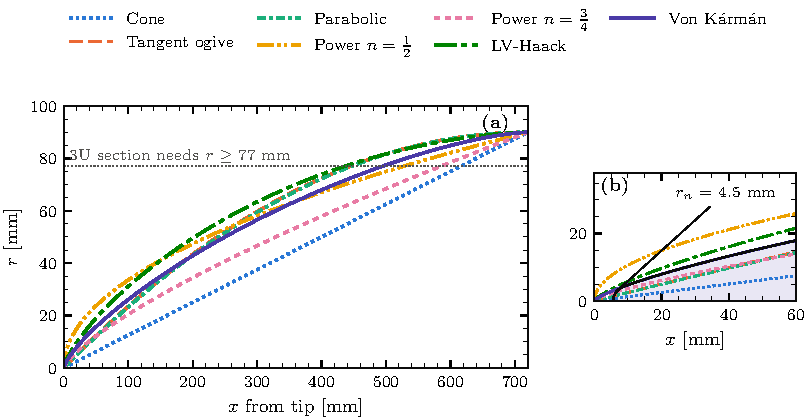
\includegraphics[width=\textwidth]{fig_profiles}
\caption{(a) The seven candidate profiles at $L/D = 4$ ($L=\SI{720}{mm}$), with the radius a 3U
section needs. (b) Tip region; the shaded profile is the Von K\'arm\'an nose with a
\SI{4.5}{mm} spherical tip ($r_n/R=0.05$) selected in Section~\ref{sec:selection}.}
\label{fig:profiles}
\end{figure}

Shapes discarded before computing: the \emph{elliptical} nose (good only subsonically; its blunt
front gives a strong bow shock above Mach 1) and the \emph{secant ogive} (no advantage over the
tangent ogive and LV-Haack at the same volume, and a slope discontinuity at the shoulder).

What matters for the comparison:
\begin{itemize}[leftmargin=*,itemsep=2pt]
\item \textbf{Wave drag.} At Weisshorn's Mach numbers (up to 1.5) the nose pressure drag
depends mostly on $L/D$ and on how much area the profile adds near the tip. Slender-body theory
gives the Von K\'arm\'an profile the minimum wave drag for given length and base area,
$C_{D,\rm w} = 1/(L/D)^2$.
\item \textbf{Volume and payload.} Fuller profiles (ogive, parabolic, LV-Haack) reach
$r=\SI{77}{mm}$ further forward, so more of the 3U unit sits inside the curved part.
\item \textbf{Stability.} The nose carries $C_{N\alpha}=2$ whatever its shape. Its centre of
pressure sits at $x_{cp}=L-V/A_b$, so a fuller nose moves the vehicle CP forward.
\item \textbf{Manufacture.} A tangent shoulder ($\theta_{\rm sh}=0$) avoids a kink at the coupler
joint. A sharp tip cannot be laid up in prepreg (ply overlaps stack at the apex), so every option
uses a separate machined tip.
\end{itemize}
